\documentclass[12pt,a4paper]{article}
\usepackage[utf8]{inputenc}
\usepackage[T1]{fontenc}
\usepackage{lmodern}
\usepackage[english]{babel}
\usepackage{geometry}
\usepackage{setspace}
\usepackage{titlesec}
\usepackage{tocloft}
\usepackage{fancyhdr}
\usepackage{graphicx}
\usepackage{float}
\usepackage{amsmath}
\usepackage{amsfonts}
\usepackage{amssymb}
\usepackage{booktabs}
\usepackage{longtable}
\usepackage{array}
\usepackage{multirow}
\usepackage{hyperref}
\usepackage{cite}
\usepackage{natbib}
\usepackage{color}
\usepackage{xcolor}
\usepackage{enumitem}
\usepackage{caption}
\usepackage{subcaption}

% Page geometry
\geometry{
    left=1in,
    right=1in,
    top=1in,
    bottom=1in,
    headheight=14pt
}

% Line spacing
\onehalfspacing

% Header and footer
\pagestyle{fancy}
\fancyhf{}
\fancyhead[L]{Digital Inclusion in Urban Communities: A Case Study}
\fancyhead[R]{\thepage}
\renewcommand{\headrulewidth}{0.4pt}

% Title formatting
\titleformat{\section}{\large\bfseries}{\thesection}{1em}{}
\titleformat{\subsection}{\normalsize\bfseries}{\thesubsection}{1em}{}
\titleformat{\subsubsection}{\normalsize\bfseries}{\thesubsubsection}{1em}{}

% Hyperlink setup
\hypersetup{
    colorlinks=true,
    linkcolor=blue,
    filecolor=magenta,      
    urlcolor=cyan,
    citecolor=red,
}

% Custom colors
\definecolor{darkblue}{RGB}{0,51,102}
\definecolor{academicgray}{RGB}{64,64,64}

\begin{document}

% Title Page
\begin{titlepage}
    \centering
    \vspace*{0.1cm}  % reduced top gap
    
    {\huge\bfseries Barriers to Digital Inclusion in Urban Communities\par}
    \vspace{0.3cm}  % less space after title
    {\Large\textit{A Case Study of E-Governance Implementation and Digital Transformation in Kathmandu Valley}\par}
    
    \vspace{1.5cm}  % space before submission info
    
    \begin{tabular}{ll}
        \textbf{Submitted to:} & Prof. Roshan Kumar Nandan \\
                               & Department of CSIT \\
        \textbf{Course:} & E-Governance \\
        \textbf{Academic Year:} & 2025 \\
    \end{tabular}
    
    \vspace{1.5cm}  % space before logo
    
    % single, properly scaled and centered logo
    \includegraphics[width=5.5cm]{logo.png}
    
    \vspace{1cm}  % space after logo
    
    % student name and email
    {\large Submitted by:\par}
    {\large Samir Paudel (79010103)\par}
    {\large Sachin Shrestha (79010099)\par}
    {\large Umesh Bogati (79010138)\par}
    
    \vspace{1cm}  % space before university info
    
    {\large Tribhuvan University\par}
    {\large Faculty of Computer Science and Information Technology\par}
    
\end{titlepage}

% Table of Contents
\newpage
\renewcommand{\contentsname}{\Large\bfseries\sffamily Table of Contents}
\tableofcontents
\newpage

% Main Content
\section{Introduction}
\label{sec:introduction}

\subsection{Background of E-Governance in Nepal}

Nepal's digital transformation journey has accelerated significantly in recent years, with the government recognizing the potential of information and communication technologies (ICTs) to improve public service delivery, enhance transparency, and promote inclusive development. The Digital Nepal Framework (DNF), first introduced in 2019 and now being revised as Digital Nepal Framework 2.0, serves as the strategic roadmap for the nation's digital transformation agenda. This framework aims to position Nepal as a digitally advanced nation by leveraging technology across all sectors—government, education, health, and commerce.

However, despite Nepal's overall broadband penetration rate of 144.56\% (as of 2024), a significant paradox exists: this high penetration does not translate into meaningful digital inclusion. Internet access and actual digital engagement remain starkly divided along geographic, socioeconomic, and demographic lines. Urban areas, particularly Kathmandu Valley, boast an internet penetration rate of 79.3\%, while rural areas languish at 17.4\%. This digital divide threatens to reinforce existing inequalities rather than bridge them.

\subsection{Importance of the Selected Topic}

The topic of ``Barriers to Digital Inclusion in Urban Communities'' is particularly relevant to Nepal for several critical reasons:

\begin{enumerate}
    \item \textbf{Paradox of Access vs. Engagement:} While urban areas theoretically have better internet access, digital literacy gaps, affordability concerns, and inadequate digital skills prevent meaningful participation in e-governance services.
    
    \item \textbf{Equity and Social Justice:} Without addressing digital inclusion barriers, e-governance initiatives risk becoming tools that primarily benefit the privileged, thereby widening the gap between different socioeconomic groups.
    
    \item \textbf{Government Service Delivery:} A significant portion of Nepal's population—including those in urban areas—cannot effectively access essential government services through digital platforms like the Nagarik App, leading to continued reliance on paper-based, time-consuming processes.
    
    \item \textbf{National Development Goals:} The Digital Nepal Framework 2.0 explicitly targets universal digital literacy and inclusive service delivery by 2030. Understanding barriers in urban areas is essential for achieving these ambitious goals.
    
    \item \textbf{Policy Relevance:} The Ministry of Communication and Information Technology (MoCIT) and the Digital Nepal Secretariat recognize digital inclusion as a cornerstone of Nepal's national development strategy, making this study directly relevant to current government priorities.
\end{enumerate}

\subsection{Purpose of the Case Study}

This case study aims to:
\begin{itemize}
    \item Understand the structural, institutional, and individual barriers that limit digital inclusion in urban communities
    \item Assess the effectiveness of current e-governance platforms (particularly the Nagarik App) in promoting digital access and service delivery
    \item Identify gaps between government intentions and ground-level implementation
    \item Document stakeholder perspectives on digital inclusion challenges
    \item Propose evidence-based recommendations for improving digital inclusion in urban areas
\end{itemize}

\subsection{Scope and Limitations}

\subsubsection{Scope}

\begin{itemize}
    \item Geographic focus: Kathmandu Valley and surrounding urban municipalities
    \item Institutional focus: Ministry of Communication and Information Technology (MoCIT) and related government agencies
    \item Thematic focus: Digital infrastructure, digital literacy, affordability, policy frameworks, and service accessibility
    \item Time period: October 2025
\end{itemize}

\subsubsection{Limitations}

\begin{itemize}
    \item This study represents a single institutional visit and may not capture the complete picture of digital inclusion challenges across all government bodies
    \item Data collected may reflect the perspectives of government officials and may differ from ground-level user experiences
    \item The study does not include extensive household surveys or community-level data collection in this phase
    \item Findings are specific to the time of visit and may change as new policies are implemented
\end{itemize}

\newpage
\section{Objectives of the Study}
\label{sec:objectives}

\subsection{Primary Objectives}

\begin{enumerate}
    \item \textbf{To evaluate the current state of digital infrastructure and services} provided by the Ministry of Communication and Information Technology in addressing digital inclusion challenges in urban communities.
    
    \item \textbf{To identify and analyze specific barriers} to digital inclusion in urban areas, including infrastructure, literacy, affordability, policy, and institutional factors.
    
    \item \textbf{To assess the effectiveness of flagship e-governance initiatives} (particularly the Nagarik App) in promoting digital access and reducing service delivery timelines.
    
    \item \textbf{To understand government strategies} for bridging the digital divide and promoting inclusive digital transformation.
\end{enumerate}

\subsection{Secondary Objectives}

\begin{enumerate}[resume]
    \item To document challenges and best practices in digital inclusion implementation.
    
    \item To explore the role of various stakeholders (government, private sector, civil society) in promoting digital inclusion.
    
    \item To gather recommendations from government officials on policy and implementation improvements.
    
    \item To contribute to the broader academic and policy discourse on digital inclusion in Nepal.
\end{enumerate}

\section{Methodology}
\label{sec:methodology}

\subsection{Research Type}

This is a \textbf{qualitative, exploratory case study} employing a combination of:
\begin{itemize}
    \item \textbf{Institutional visit and observation:} Direct observation of the Ministry's operations and digital initiatives
    \item \textbf{Stakeholder interviews:} Structured and semi-structured interviews with government officials
    \item \textbf{Document review:} Analysis of policy documents, framework documents, and project reports
    \item \textbf{Field notes:} Observations of infrastructure, office setups, and service delivery mechanisms
\end{itemize}

\subsection{Research Tools and Data Collection Methods}

\begin{enumerate}
    \item \textbf{Interview Schedule:} Structured questionnaire for officials (see Annexure A)
    \begin{itemize}
        \item Questions focused on digital infrastructure, service delivery, user feedback, and challenges
        \item Topics: Government initiatives, barriers identified, success metrics, recommendations
    \end{itemize}
    
    \item \textbf{Observation Checklist:} For assessing physical infrastructure and digital facilities
    \begin{itemize}
        \item Internet connectivity quality
        \item Digital devices and systems available
        \item Office organization and service delivery setup
    \end{itemize}
    
    \item \textbf{Document Collection and Review:}
    \begin{itemize}
        \item Digital Nepal Framework 2.0 (draft and conceptual documents)
        \item Nagarik App documentation and user statistics
        \item Project briefs on e-governance initiatives
    \end{itemize}
    
    \item \textbf{Photography/Annotated Images:} Visual documentation of infrastructure and systems (with permission)
\end{enumerate}

\subsection{Sample and Respondents}

\begin{itemize}
    \item \textbf{Primary Respondent Institution:} Ministry of Communication and Information Technology (MoCIT), Kathmandu
    \item \textbf{Number of Officials Interviewed:} 3-5 officials, including IT coordinators, policy officers, and Nagarik App team members
    \item \textbf{Other Stakeholders Consulted:} Digital Nepal Secretariat officials, National Information Technology Center (NITC) representatives
\end{itemize}

\subsection{Duration and Timeline}

\begin{itemize}
    \item \textbf{Field Visit Date:} October 23, 2025
    \item \textbf{Pre-Visit Preparation:} October 15-22, 2025 (literature review, questionnaire development)
    \item \textbf{Post-Visit Analysis:} October 24-31, 2025 (data transcription, analysis, report writing)
\end{itemize}

\newpage
\section{Organizational Overview}
\label{sec:organization}

\subsection{Ministry of Communication and Information Technology (MoCIT)}

\subsubsection{History and Mandate}

The Ministry of Communication and Information Technology (MoCIT) is the apex government body responsible for formulating policies, strategies, and programs related to information and communication technologies in Nepal. Established with the broader mandate to accelerate Nepal's digital transformation, MoCIT oversees:

\begin{itemize}
    \item \textbf{E-governance initiatives:} Development and implementation of digital platforms for government service delivery
    \item \textbf{Digital infrastructure:} Planning for broadband expansion, data centers, and cybersecurity
    \item \textbf{Digital policy and legislation:} Drafting and implementation of ICT-related laws and frameworks
    \item \textbf{Capacity building:} Training and development programs for government employees and the public
    \item \textbf{National coordination:} Serving as the nodal agency for the Digital Nepal Framework
\end{itemize}

\subsubsection{Organization Structure}

MoCIT operates through several key divisions:
\begin{itemize}
    \item \textbf{E-governance Division:} Oversees digital service platforms and integration
    \item \textbf{ICT Infrastructure Division:} Manages broadband policy and digital infrastructure development
    \item \textbf{Digital Literacy and Inclusion Division:} Coordinates digital literacy programs (new division under DNF 2.0)
    \item \textbf{Cybersecurity and Data Protection Division:} Ensures secure digital ecosystems
    \item \textbf{Technical Support Unit (National Information Technology Center - NITC):} Provides technical backend support for government digital systems
\end{itemize}

\subsubsection{Key Services and Initiatives Offered}

\begin{enumerate}
    \item \textbf{Nagarik App:} An integrated mobile platform providing over 200+ government services including:
    \begin{itemize}
        \item PAN registration and tax filing
        \item Citizenship and passport services
        \item Vehicle registration and tax payments
        \item Business licensing and permits
        \item Banking and financial service integration
    \end{itemize}
    
    \item \textbf{Digital Public Infrastructure (DPI):}
    \begin{itemize}
        \item National ID and digital identity services
        \item Unified payment interfaces
        \item Digital signature and authentication systems
    \end{itemize}
    
    \item \textbf{E-Governance Project (World Bank-Supported):}
    \begin{itemize}
        \item Modernizing government service delivery
        \item Integrating systems across ministries
        \item Implementing Business Process Reengineering (BPR)
    \end{itemize}
    
    \item \textbf{Digital Literacy Initiatives:}
    \begin{itemize}
        \item ICT Gyan provincial campaign (launched May 2025, completed across all 7 provinces)
        \item Training programs for government employees
        \item Public awareness campaigns
    \end{itemize}
    
    \item \textbf{National Broadband Policy Implementation:}
    \begin{itemize}
        \item Expanding fiber optic networks
        \item Promoting public-private partnerships
        \item Targeting universal high-speed internet access by 2030
    \end{itemize}
\end{enumerate}

\section{Description of E-Governance Systems and Digital Inclusion Initiatives}

\subsection{The Nagarik App: Digital Nepal's Flagship Platform}

\subsubsection{Overview and Features}

The Nagarik App, launched by the Government of Nepal under MoCIT's coordination, represents Nepal's most ambitious attempt to create a single digital window for government service delivery. The app is available on both iOS and Android platforms and has been downloaded by over 625,000 users, with more than 200,000 verified users (as of 2021).

\subsubsection{Key Features}

\begin{enumerate}
    \item \textbf{Integrated Service Delivery:}
    \begin{itemize}
        \item Citizen Information and Verification
        \item Tax and revenue services
        \item Local government services
        \item Integrated Digital Identity (leveraging National ID data)
    \end{itemize}
    
    \item \textbf{Technology Stack:}
    \begin{itemize}
        \item Mobile-first design (both app and web portal)
        \item API-based integration with government systems
        \item Secure data transmission protocols
        \item Digital signature support
    \end{itemize}
    
    \item \textbf{Target Users:}
    \begin{itemize}
        \item General citizens accessing government services
        \item Businesses for licensing and compliance
        \item Government employees coordinating service delivery
    \end{itemize}
\end{enumerate}

\subsubsection{Current Service Coverage}

The Nagarik App currently integrates services from multiple government agencies:
\begin{itemize}
    \item \textbf{Revenue Services:} Tax filing, PAN registration, vehicle tax payment
    \item \textbf{Identification:} Citizenship verification, police clearance certificates
    \item \textbf{Local Government:} Ward services, local permits, property information
    \item \textbf{Social Services:} Health insurance enrollment, social protection schemes
    \item \textbf{Financial Services:} Bank account opening with digital verification
\end{itemize}

\subsubsection{Expansion Plans}

Under the Digital Nepal Framework 2.0 and the World Bank-supported Nepal Digital Transformation Project:
\begin{itemize}
    \item 80+ new services to be added by 2026
    \item Integration with district-level services
    \item Enhanced public-private partnerships for expanded service delivery
    \item Improved backend system integration for end-to-end digitization
\end{itemize}

\subsection{Other Key E-Governance Initiatives}

\subsubsection{Digital Public Infrastructure (DPI)}

\textbf{National ID System:}
\begin{itemize}
    \item Biometric-based identification system with 15.5 million citizen records
    \item Serves as the foundational layer for digital service delivery
    \item Enables digital signature and authentication across platforms
\end{itemize}

\textbf{Data Centers and Secure Infrastructure:}
\begin{itemize}
    \item Modernization of government data hosting facilities
    \item Implementation of cybersecurity protocols
    \item Establishment of disaster recovery and business continuity mechanisms
\end{itemize}

\subsubsection{Digital Literacy and Inclusion Programs}

\textbf{ICT Gyan Initiative (May 2025 - Present):}
\begin{itemize}
    \item Joint initiative of ICT Foundation Nepal and Ncell Foundation
    \item Target: 2,000+ participants across all 7 provinces
    \item Focus areas:
    \begin{itemize}
        \item Safe internet use and cybercrime awareness
        \item Digital literacy for young people and women
        \item Career skill development in digital domains
    \end{itemize}
\end{itemize}

\textbf{Government Employee Digital Competency Program:}
\begin{itemize}
    \item Training civil servants in digital tools and platforms
    \item Building capacity for digital transformation implementation
    \item Expected to prepare 40,000+ government employees by 2026
\end{itemize}

\subsubsection{National Broadband Expansion}

\textbf{Strategic Partnerships (2025):}
\begin{itemize}
    \item IFC-Standard Chartered Bank-WorldLink Communications partnership: \$29 million investment
    \item Target: Expand fiber networks to underserved urban and peri-urban areas
    \item Expected outcomes:
    \begin{itemize}
        \item Enhanced connectivity in remote urban colonies
        \item Improved service quality for existing users
        \item Job creation through infrastructure development
    \end{itemize}
\end{itemize}

\newpage
\section{Key Observations and Findings}
\label{sec:findings}

\subsection{Observation 1: The Paradox of High Access, Low Engagement}

\textbf{Finding:} While Kathmandu Valley reports 79.3\% internet penetration, actual usage of e-government services remains significantly lower than expected. According to data reviewed from government reports, awareness of the Nagarik App is high in urban areas, but actual usage rates tell a different story. Only a fraction of those who download the app proceed to verify their identity and use integrated services.

\textbf{Evidence from Field Visit:}
\begin{itemize}
    \item MoCIT officials acknowledged that ``awareness is high, but actual usage is a challenge''
    \item Digital literacy gaps persist even among urban populations with internet access
    \item Many users lack the skills or confidence to navigate digital government platforms
\end{itemize}

\subsection{Observation 2: Digital Literacy as the Critical Barrier}

\textbf{Finding:} The gap between general literacy (76\% nationally) and digital literacy (31\% nationally) represents the single greatest barrier to digital inclusion. In urban areas, while literacy rates are higher, digital literacy—the ability to effectively use digital tools for meaningful purposes—remains limited.

\textbf{Key Statistics Identified:}
\begin{itemize}
    \item Only 31\% of Nepal's population possesses functional digital literacy skills
    \item Many urban residents use the internet primarily for social media and entertainment, not government services
    \item Limited awareness of how to use government digital platforms
    \item Generational and gender disparities in digital competency (women lag significantly behind men)
\end{itemize}

\textbf{Observations During Visit:}
\begin{itemize}
    \item MoCIT officials highlighted digital literacy as the ``most significant predictor'' of Nagarik App usage
    \item Government is launching targeted training programs but acknowledges limited resources and outreach
    \item Awareness campaigns have been passive; more active, community-based approaches are needed
\end{itemize}

\subsection{Observation 3: Fragmented Back-End Systems Limit Service Delivery}

\textbf{Finding:} While the Nagarik App presents a user-friendly front-end interface, many government services remain hampered by non-integrated, paper-based back-end processes.

\textbf{Specific Examples Noted:}
\begin{itemize}
    \item Citizenship verification may be completed online, but document issuance still requires physical office visits
    \item Tax filing is digitized at the front-end, but approval and credential issuance remain manual
    \item Integration between different government departments is incomplete, creating data silos
\end{itemize}

\textbf{Impact on Digital Inclusion:}
\begin{itemize}
    \item Users cannot experience the full benefits of ``one-stop government'' service
    \item Time-saving advantages are minimal when manual steps persist
    \item Citizens must maintain parallel digital and physical service pathways
\end{itemize}

\subsection{Observation 4: Trust Deficit and Data Security Concerns}

\textbf{Finding:} Public hesitancy to share personal data with government platforms remains a significant barrier, rooted in:
\begin{itemize}
    \item Inadequate data protection legal frameworks
    \item Historical instances of government data breaches
    \item General concerns about surveillance and misuse of personal information
\end{itemize}

\textbf{Evidence from Government Reports Reviewed:}
\begin{itemize}
    \item Nepal's data protection law falls below international standards
    \item This trust deficit suppresses adoption of e-governance services
    \item Citizens are hesitant to provide biometric data and personal information online
\end{itemize}

\textbf{Implications for Digital Inclusion:}
\begin{itemize}
    \item Even when digital infrastructure and literacy exist, trust barriers prevent service adoption
    \item Building trust requires not just technological investment but legal and institutional reforms
\end{itemize}

\subsection{Observation 5: Gender and Socioeconomic Disparities Within Urban Areas}

\textbf{Finding:} Digital inclusion in urban Kathmandu is not uniform. Significant disparities exist based on:
\begin{itemize}
    \item \textbf{Gender:} Women face additional barriers (socio-cultural factors, limited mentorship, cybersecurity concerns)
    \item \textbf{Socioeconomic Status:} Low-income urban households in informal settlements have limited device access and internet affordability
    \item \textbf{Age:} Elderly population remains largely excluded from digital services
\end{itemize}

\textbf{Statistical Context Gathered:}
\begin{itemize}
    \item UN Women reports indicate that gender digital gaps could cost Nepal Rs 15 billion by 2025
    \item Women make up only 43.6\% of Nepal's social media users, and participation in digital government services is even lower
    \item Online harassment and cyber threats disproportionately affect women
\end{itemize}

\textbf{Observations:}
\begin{itemize}
    \item MoCIT recognizes these disparities but limited gender-specific interventions have been implemented
    \item Recent policy discussions (November 2025) included explicit commitment to gender-sensitive digital inclusion
\end{itemize}

\subsection{Observation 6: Infrastructure Limitations in Peri-Urban Areas}

\textbf{Finding:} While Kathmandu proper has reasonable connectivity, peri-urban settlements and informal colonies face:
\begin{itemize}
    \item Unreliable electricity supply
    \item Limited broadband coverage
    \item Lower device penetration among lower-income populations
\end{itemize}

\textbf{Policy Response Noted:}
\begin{itemize}
    \item World Bank-supported Nepal Digital Transformation Project acknowledges need for targeted infrastructure investment
    \item Plans to ensure accessibility for persons with disabilities
    \item Focus on underserved urban neighborhoods in digital infrastructure expansion plans
\end{itemize}

\subsection{Observation 7: Institutional and Policy Progress}

\textbf{Positive Findings:}
\begin{itemize}
    \item Strong government commitment to digital inclusion (evidenced by Digital Nepal Framework 2.0 revision)
    \item Recognition of digital literacy as a key strategic area
    \item Institutional coordination mechanisms being established (Digital Coordination Unit under new projects)
    \item Private-sector partnerships expanding to supplement government efforts
\end{itemize}

\textbf{Challenges Acknowledged:}
\begin{itemize}
    \item Fragmented approach across government agencies (despite improving coordination)
    \item Limited dedicated budget for digital literacy programs
    \item Insufficient human resources in implementation agencies
    \item Coordination gaps between national, provincial, and local government levels
\end{itemize}

\newpage
\section{Analysis and Discussion}
\label{sec:analysis}

\subsection{The Digital Divide Within Urban Areas}

While national-level statistics show Kathmandu Valley's 79.3\% internet penetration as significantly higher than rural areas' 17.4\%, this aggregate figure masks important within-urban disparities. Our analysis reveals a \textbf{stratified digital divide} within urban communities:

\vspace{6pt}
\noindent\textbf{Tier 1: Digitally Included (Upper Urban Class)}
\begin{itemize}[leftmargin=1.5em]
    \item High-speed internet access at home and work
    \item Multiple devices (computer, smartphone, tablet)
    \item High digital literacy and online safety awareness
    \item Active users of government digital platforms
    \item Estimated proportion: 25-30\% of urban population
\end{itemize}

\vspace{6pt}
\noindent\textbf{Tier 2: Partially Included (Middle Urban Class)}
\begin{itemize}[leftmargin=1.5em]
    \item Internet access through smartphones primarily
    \item One or two devices per household
    \item Moderate digital literacy; comfortable with social media but uncertain about government platforms
    \item Potential users of e-services with awareness and support
    \item Estimated proportion: 40-45\% of urban population
\end{itemize}

\vspace{6pt}
\noindent\textbf{Tier 3: Digitally Excluded (Lower Urban Class)}
\begin{itemize}[leftmargin=1.5em]
    \item Limited internet access (reliant on neighborhood WiFi or data plans)
    \item Device constraints; shared or outdated devices
    \item Low digital literacy; unfamiliarity with government platforms
    \item Limited access to digital services; continued reliance on manual processes
    \item Estimated proportion: 25-35\% of urban population
\end{itemize}

\subsection{Root Cause Analysis: The Multifaceted Barriers}

Using a systems-thinking approach, we identify interconnected barriers to digital inclusion:

\subsubsection{1. Infrastructure Barriers}

\textbf{Despite high penetration, quality of connectivity varies significantly}
\begin{itemize}
    \item Urban fiber optic networks benefit only central districts
    \item Peri-urban areas rely on mobile data or slower connections
    \item Power supply inconsistencies affect sustained digital service use
\end{itemize}

\textbf{Mitigation Efforts:} IFC-Standard Chartered-WorldLink partnership aims to expand to underserved areas; however, investment is insufficient for comprehensive coverage

\subsubsection{2. Economic Barriers}

\textbf{Affordability remains a critical concern even in urban areas}
\begin{itemize}
    \item Device costs (smartphones: \$100-400; computers: \$300-1000) are prohibitive for lower-income households
    \item Internet data costs accumulate significantly for regular service use
    \item Data costs for accessing government platforms accumulate
\end{itemize}

\textbf{Policy Response:} Free WiFi initiatives in public spaces (ongoing); device subsidy programs (limited)

\subsubsection{3. Capacity and Skills Barriers}

\textbf{Digital literacy deficits prevent meaningful engagement}
\begin{itemize}
    \item Users cannot navigate complex government digital interfaces
    \item Limited understanding of digital security and privacy protection
    \item Lack of problem-solving skills when digital services fail
    \item Language barriers (many platforms only in Nepali; limited accessibility for marginalized language speakers)
\end{itemize}

\textbf{Government Response:} ICT Gyan program reaching 2,000+ people; plans for targeted literacy initiatives; need for scaling and sustainability

\subsubsection{4. Institutional and Design Barriers}

\textbf{Government digital platforms not designed with user inclusion in mind}
\begin{itemize}
    \item Complex interfaces assuming high digital literacy
    \item Inadequate user support and help systems
    \item Limited accessibility for persons with disabilities
    \item Offline/alternative service pathways not clearly communicated
\end{itemize}

\textbf{Organizational Weakness:} Fragmented backend systems requiring manual verification steps, undermining the benefits of digital frontends

\subsubsection{5. Trust and Security Barriers}

\textbf{Low institutional trust suppresses adoption despite good digital infrastructure}
\begin{itemize}
    \item Data protection law inadequate
    \item Historical instances of data breaches and misuse
    \item Concerns about government surveillance and privacy
    \item Lack of transparent data governance policies
\end{itemize}

\textbf{Impact:} Even tech-literate users hesitant to provide personal data and biometric information

\subsubsection{6. Gender and Social Inclusion Barriers}

\textbf{Digital inclusion is not gender-neutral}
\begin{itemize}
    \item Socio-cultural norms restrict women's technology access
    \item Online harassment and cybersecurity threats disproportionately affect women
    \item Lower digital literacy rates among women
    \item Intersectional exclusion of women from marginalized communities
\end{itemize}

\textbf{Policy Recognition:} Recent government consultations (November 2025) identified these gaps; integration of gender considerations in Digital Nepal Framework 2.0 ongoing

\subsection{Comparison of Intended Outcomes vs. Actual Outcomes}

\begin{table}[ht]
\centering
\small
\caption{Comparison of Intended vs. Actual Outcomes}
\vspace{6pt}
\begin{tabular}{@{}p{4.2cm}p{4.2cm}p{4.8cm}@{}}
\toprule
\textbf{Intended Outcome} & \textbf{Actual Outcome} & \textbf{Gap Analysis} \\
\textbf{(Digital Nepal Vision)} & \textbf{(Ground Reality)} & \\
\midrule
Universal access to government services through digital platforms & Limited service usage; many still use manual processes & High digital literacy and trust still required \\
\addlinespace
Significant time savings through digitization & Minimal time savings due to non-integrated backend systems & End-to-end digitization incomplete \\
\addlinespace
Reduced social inequality through digital access & Risk of widening inequality; digital benefits concentrated among privileged & Inclusion not automatic; requires deliberate intervention \\
\addlinespace
31\% digital literacy → 90\% by 2029 (government goal) & Current literacy unchanged; awareness growing but skills lag & Aggressive literacy programs needed; current pace insufficient \\
\addlinespace
Elimination of paper-based government processes & Paper processes persist in approval and verification stages & Process reengineering incomplete; organizational inertia high \\
\bottomrule
\end{tabular}
\end{table}

\subsection{Alignment with Digital Nepal Framework Objectives}

\textbf{Areas of Alignment:}
\begin{itemize}
    \item MoCIT's strategic focus on digital literacy addresses identified barriers
    \item Nagarik App represents thoughtful platform design for service integration
    \item Recognition of inclusion as explicit objective in DNF 2.0
    \item Private-sector partnerships addressing infrastructure gaps
\end{itemize}

\textbf{Areas Requiring Strengthening:}
\begin{itemize}
    \item Pace of digital literacy intervention insufficient for scale of need
    \item Limited focus on gender and social inclusion in implementation
    \item Institutional coordination gaps between national and local levels
    \item Trust-building measures (legal reforms, transparency) lagging behind platform development
\end{itemize}

\newpage
\section{Conclusion}
\label{sec:conclusion}

\subsection{Summary of Key Findings}

The case study reveals a paradox at the heart of Nepal's urban digital transformation: high internet penetration coexists with low digital inclusion. The Ministry of Communication and Information Technology has launched ambitious initiatives, particularly the Nagarik App and the Digital Nepal Framework 2.0, which represent sophisticated policy thinking and technical achievement. However, ground-level barriers—spanning digital literacy, trust, institutional capacity, and social factors—prevent these platforms from achieving their inclusive potential.

Digital inclusion in urban Kathmandu is not simply a matter of providing internet access and digital platforms. Rather, it requires simultaneous attention to:
\begin{enumerate}
    \item Building digital literacy skills appropriate to diverse population segments
    \item Establishing trust through robust data protection and transparent governance
    \item Redesigning government processes for end-to-end digitization
    \item Explicitly addressing gender, socioeconomic, and age-based disparities
    \item Ensuring accessibility for persons with disabilities and marginalized communities
\end{enumerate}

\subsection{Lessons Learned}

\textbf{Lesson 1: Access Alone Is Insufficient}

High internet penetration does not guarantee digital inclusion. Digital literacy, affordability, trust, and institutional design are equally critical. Policy and investment must address all dimensions simultaneously.

\textbf{Lesson 2: Digital Transformation Is Fundamentally Organizational}

Technology platforms fail without corresponding organizational reforms. The persistence of manual backend processes undermines the Nagarik App's potential benefits. Digital transformation requires Business Process Reengineering at the institutional level.

\textbf{Lesson 3: Inclusion Requires Intentional Design}

Digital platforms, if designed without explicit inclusion principles, will reinforce existing inequalities. Gender, socioeconomic status, disability, and language must be explicit considerations in system design and implementation, not afterthoughts.

\textbf{Lesson 4: Trust Is Foundational}

Public hesitancy to share data with government platforms reflects rational concerns about data protection and privacy. Building trust requires not just technological investment but legal reforms, transparent governance, and demonstrated institutional commitment to citizen rights.

\textbf{Lesson 5: Institutional Capacity and Coordination Matter}

Fragmented government systems undermine digital transformation efforts. Successful implementation requires strong coordination mechanisms, clear institutional roles, and adequate human resource capacity across all levels of government.

\subsection{Overall Assessment of System Effectiveness}

\textbf{Current State:} The Nagarik App and associated e-governance initiatives represent a strong strategic foundation and demonstrate Nepal's commitment to digital transformation. The platform is well-designed, technically sound, and serves as an important entry point for digital government services.

\textbf{Effectiveness for Digital Inclusion:} However, effectiveness in promoting inclusive digital engagement remains limited. While digitally literate, urban, middle and upper-class residents benefit substantially, lower-income populations and those with lower digital literacy remain largely excluded. The platform thus risks becoming a tool that serves the already-privileged rather than catalyzing broad-based digital inclusion.

\textbf{Outlook:} With sustained commitment to the identified barriers—particularly digital literacy at scale, institutional reforms, and explicit inclusion measures—the platforms and frameworks being deployed have significant potential to advance digital inclusion. The government's revised Digital Nepal Framework 2.0 and World Bank partnership suggest strengthened commitment to these challenges.

\newpage
\section{Recommendations}
\label{sec:recommendations}

\subsection{For Policy Makers and Government Leadership}

\subsubsection{1. Scale Digital Literacy Interventions Dramatically}

\textbf{Action:} Establish a National Digital Literacy Commission with dedicated budget (minimum Rs. 5 billion annually)

\textbf{Target:} Achieve 60\% functional digital literacy by 2027 (from current 31\%)

\textbf{Approach:} Move beyond awareness campaigns to hands-on, community-based literacy programs in all urban neighborhoods

\textbf{Specifics:}
\begin{itemize}
    \item Partner with schools, libraries, and community centers for free training
    \item Develop age-appropriate and context-specific training modules
    \item Integrate digital literacy into secondary school curriculum nationwide
\end{itemize}

\subsubsection{2. Strengthen Legal Frameworks for Data Protection and Privacy}

\textbf{Action:} Enact a comprehensive Data Protection Law meeting international standards within 2026

\textbf{Rationale:} Address public trust deficits preventing adoption of government digital platforms

\textbf{Implementation:}
\begin{itemize}
    \item Establish an independent Data Protection Authority
    \item Implement transparent data governance policies
    \item Conduct public awareness on data rights and protections
\end{itemize}

\subsubsection{3. Mandate End-to-End Digital Service Transformation}

\textbf{Action:} Require all government agencies to complete Business Process Reengineering (BPR) for integration with Nagarik App

\textbf{Timeline:} Baseline mapping by June 2026; full integration by December 2027

\textbf{Focus:} Move beyond digitizing front-end forms to fully automating back-office verification, approval, and issuance processes

\textbf{Accountability:} Link budget allocations to BPR completion metrics

\subsubsection{4. Establish Explicit Gender and Inclusion Targets}

\textbf{Action:} Integrate gender and social inclusion targets into Digital Nepal Framework 2.0 implementation

\textbf{Targets (by 2027):}
\begin{itemize}
    \item 50\% of Nagarik App users must be women
    \item 75\% digital literacy among women in urban areas
    \item Language diversity: Services available in minimum 5 languages
\end{itemize}

\textbf{Implementation:}
\begin{itemize}
    \item Women-focused digital literacy programs in partnership with women's organizations
    \item Safety and cybersecurity training addressing women's concerns
    \item Address childcare barriers to women's participation in training
\end{itemize}

\subsubsection{5. Strengthen Intergovernmental Coordination}

\textbf{Action:} Establish a Digital Transformation Coordinating Committee with representation from federal, provincial, and local governments

\textbf{Function:}
\begin{itemize}
    \item Ensure alignment of digital initiatives across all levels
    \item Facilitate resource sharing and technical support
    \item Monitor inclusion metrics at all government levels
\end{itemize}

\textbf{Oversight:} Chaired by MoCIT with explicit accountability to the Planning Commission

\subsection{For Implementation Agencies}

\subsubsection{6. Adopt Universal Design Principles}

\textbf{Platform Design:}
\begin{itemize}
    \item Simplify user interfaces with step-by-step guidance
    \item Provide multi-lingual support (Nepali, English, major regional languages)
    \item Ensure accessibility for persons with disabilities (screen readers, visual aids)
    \item Include offline fallback options for low-connectivity areas
\end{itemize}

\subsubsection{7. Establish Citizen Support Infrastructure}

\textbf{Digital Service Centers:}
\begin{itemize}
    \item Create neighborhood digital service centers in all urban municipalities
    \item Staff with trained assistants to help citizens navigate digital platforms
    \item Provide free device access and internet connectivity
    \item Offer on-site training and troubleshooting
\end{itemize}

\subsubsection{8. Implement Continuous User Feedback Mechanisms}

\textbf{Feedback Systems:}
\begin{itemize}
    \item Regular user satisfaction surveys
    \item In-app feedback and rating mechanisms
    \item Community focus groups with diverse population segments
    \item Rapid response protocols for user complaints and issues
\end{itemize}

\subsection{For Development Partners and Civil Society}

\subsubsection{9. Support Community-Based Digital Literacy Programs}

\textbf{Role for NGOs and Civil Society:}
\begin{itemize}
    \item Partner with government for grassroots literacy training
    \item Develop culturally appropriate training materials
    \item Reach marginalized communities (women, elderly, persons with disabilities)
    \item Provide mentorship and peer-learning opportunities
\end{itemize}

\subsubsection{10. Advocate for Inclusive Policy and Accountability}

\textbf{Advocacy Priorities:}
\begin{itemize}
    \item Monitor government compliance with inclusion targets
    \item Document and publicize success stories and challenges
    \item Amplify voices of excluded communities in policy discussions
    \item Support independent research on digital inclusion impacts
\end{itemize}

\subsection{For Private Sector Partners}

\subsubsection{11. Expand Affordable Connectivity Solutions}

\textbf{Telecommunications Companies:}
\begin{itemize}
    \item Offer subsidized data plans for government service access
    \item Expand network coverage to peri-urban areas
    \item Provide zero-rated access to government portals (no data charges)
    \item Support community WiFi initiatives in underserved neighborhoods
\end{itemize}

\subsubsection{12. Device Affordability Programs}

\textbf{Technology Providers:}
\begin{itemize}
    \item Develop low-cost smartphone models suitable for government services
    \item Offer installment payment plans for devices
    \item Partner with government for device subsidy programs
    \item Support device recycling and refurbishment programs
\end{itemize}

\newpage
\section{References}

\begin{thebibliography}{20}

\bibitem{DivaPortal2025}
\textit{Bridging the Digital Divide in Nepal's E-Government}. DiVA Portal, Digital Academic Archive.
\href{https://www.diva-portal.org/smash/record.jsf?pid=diva2\%3A1977098&dswid=-5328}{https://www.diva-portal.org/...}

\bibitem{NepaliTelecom2025}
Nepali Telecom. \textit{The State of Digital Divide in Nepal and How to Reduce It}. 
\href{https://www.nepalitelecom.com/digital-divide}{https://www.nepalitelecom.com/...}

\bibitem{DigitalRightsNepal2024}
Digital Rights Nepal. (2024). \textit{State of Digital Rights and Safety in Nepal 2024}. 
\href{https://digitalrightsnepal.org/wp-content/uploads/2025/05/STATE-OF-DIGITAL-RIGHTS-AND-SAFETY-IN-NEPAL-2024-1-1-2.pdf}{https://digitalrightsnepal.org/...}

\bibitem{MyRepublica2025}
My Republica (Nagarik Network). \textit{E-Governance in Nepal: Challenges and Opportunities}. 
\href{https://myrepublica.nagariknetwork.com/news/e-governance-in-nepal-challenges-and-opportunities-95-85.html}{https://myrepublica.nagariknetwork.com/...}

\bibitem{HimalayanTimes2025}
The Himalayan Times. (2025). \textit{Nepal's Persistent Digital Divide: From High Penetration to Inclusion}. 
\href{https://thehimalayantimes.com/opinion/nepals-persistent-digital-divide-from-high-penetration-to-inclusion}{https://thehimalayantimes.com/...}

\end{thebibliography}

\vspace{12pt}

\noindent\textit{Note:} this case study mainly focuses on the field visit to the ministry of communication and information technology (mocit); however, additional government researches, policy documents, online resources were used to refine and support the analysis.


\newpage
\section{Annexures}
\label{sec:annexures}

\subsection{Annexure A: Interview Questions for Government Officials}

\subsubsection{Section 1: Digital Infrastructure and Service Delivery}

\begin{enumerate}
    \item What digital services does your ministry/department currently offer to citizens?
    \item How would you assess the current state of digital infrastructure supporting these services?
    \item What are the main technical challenges you face in service delivery?
    \item How do you measure the success and adoption of digital services?
\end{enumerate}

\subsubsection{Section 2: Digital Inclusion and Barriers}

\begin{enumerate}[resume]
    \item What do you perceive as the main barriers preventing citizens from using digital government services?
    \item Have you observed differences in digital service adoption across different demographic groups (age, gender, income)?
    \item What feedback do you receive from citizens regarding digital services?
    \item Are there specific populations that remain excluded from digital services?
\end{enumerate}

\subsubsection{Section 3: Policy and Strategy}

\begin{enumerate}[resume]
    \item How does your organization's digital strategy align with the Digital Nepal Framework?
    \item What specific initiatives are underway to promote digital inclusion?
    \item What resources (budget, personnel, technology) are allocated for digital inclusion?
    \item How do you coordinate with other government agencies on digital transformation?
\end{enumerate}

\subsubsection{Section 4: Recommendations and Future Plans}

\begin{enumerate}[resume]
    \item What improvements would you recommend for current digital service delivery?
    \item What are your organization's priorities for the next 2-3 years in digital inclusion?
    \item What support (from government, private sector, or development partners) would most help advance digital inclusion?
    \item What lessons have you learned from digital transformation efforts so far?
\end{enumerate}

\subsection{Annexure B: Observation Checklist}

\subsubsection{Infrastructure Assessment}

\begin{itemize}
    \item[$\square$] Internet connectivity quality (speed, reliability)
    \item[$\square$] Digital devices available (computers, tablets, smartphones)
    \item[$\square$] Server and data center infrastructure
    \item[$\square$] Backup power supply systems
    \item[$\square$] Network security measures visible
\end{itemize}

\subsubsection{Service Delivery Setup}

\begin{itemize}
    \item[$\square$] Citizen service counters and digital kiosks
    \item[$\square$] Digital display boards and information systems
    \item[$\square$] Help desk and support systems
    \item[$\square$] Document digitization systems
    \item[$\square$] Queue management systems
\end{itemize}

\subsubsection{Accessibility Features}

\begin{itemize}
    \item[$\square$] Wheelchair accessibility
    \item[$\square$] Multi-lingual signage and interfaces
    \item[$\square$] Assistive technologies for persons with disabilities
    \item[$\square$] Separate facilities for women and children
    \item[$\square$] Privacy protection measures
\end{itemize}

\subsection{Annexure C: Key Statistics Summary}

\vspace{12pt}

\begin{table}[H]
\centering
\caption{Key Statistics on Digital Inclusion in Nepal}
\vspace{8pt}
\begin{tabular}{@{}p{8cm}r@{}}
\toprule
\textbf{Metric} & \textbf{Value} \\
\midrule
\multicolumn{2}{@{}l}{\textit{\textbf{Internet and Digital Access}}} \\
\addlinespace[3pt]
National broadband penetration & 144.56\% \\
Urban internet penetration & 79.3\% \\
Rural internet penetration & 17.4\% \\
National digital literacy rate & 31\% \\
National general literacy rate & 76\% \\
\addlinespace[6pt]
\multicolumn{2}{@{}l}{\textit{\textbf{Nagarik App and Digital Services}}} \\
\addlinespace[3pt]
Nagarik App downloads & 625,000+ \\
Nagarik App verified users & 200,000+ \\
National ID records & 15.5 million \\
Services on Nagarik App & 200+ \\
\addlinespace[6pt]
\multicolumn{2}{@{}l}{\textit{\textbf{Training and Capacity Building}}} \\
\addlinespace[3pt]
ICT Gyan training participants & 2,000+ \\
Government employees to be trained & 40,000+ \\
Women in social media users & 43.6\% \\
\bottomrule
\end{tabular}
\end{table}

\vspace{12pt}

\subsection{Annexure D: Field Visit Documentation}

\subsubsection{Figure 1: Field Visit Approval Letter}

\begin{figure}[H]
\centering

\includegraphics[width=0.75\textwidth]{letter.png}
\caption{Official recommendation letter from Tribhuvan University, Patan Multiple Campus for field visit to Ministry of Communication and Information Technology (Ref. No. 06/082, dated October 10, 2025)}
\end{figure}

\subsubsection{Figure 2: Ministry of Communication and Information Technology Building}

\begin{figure}[H]
\centering
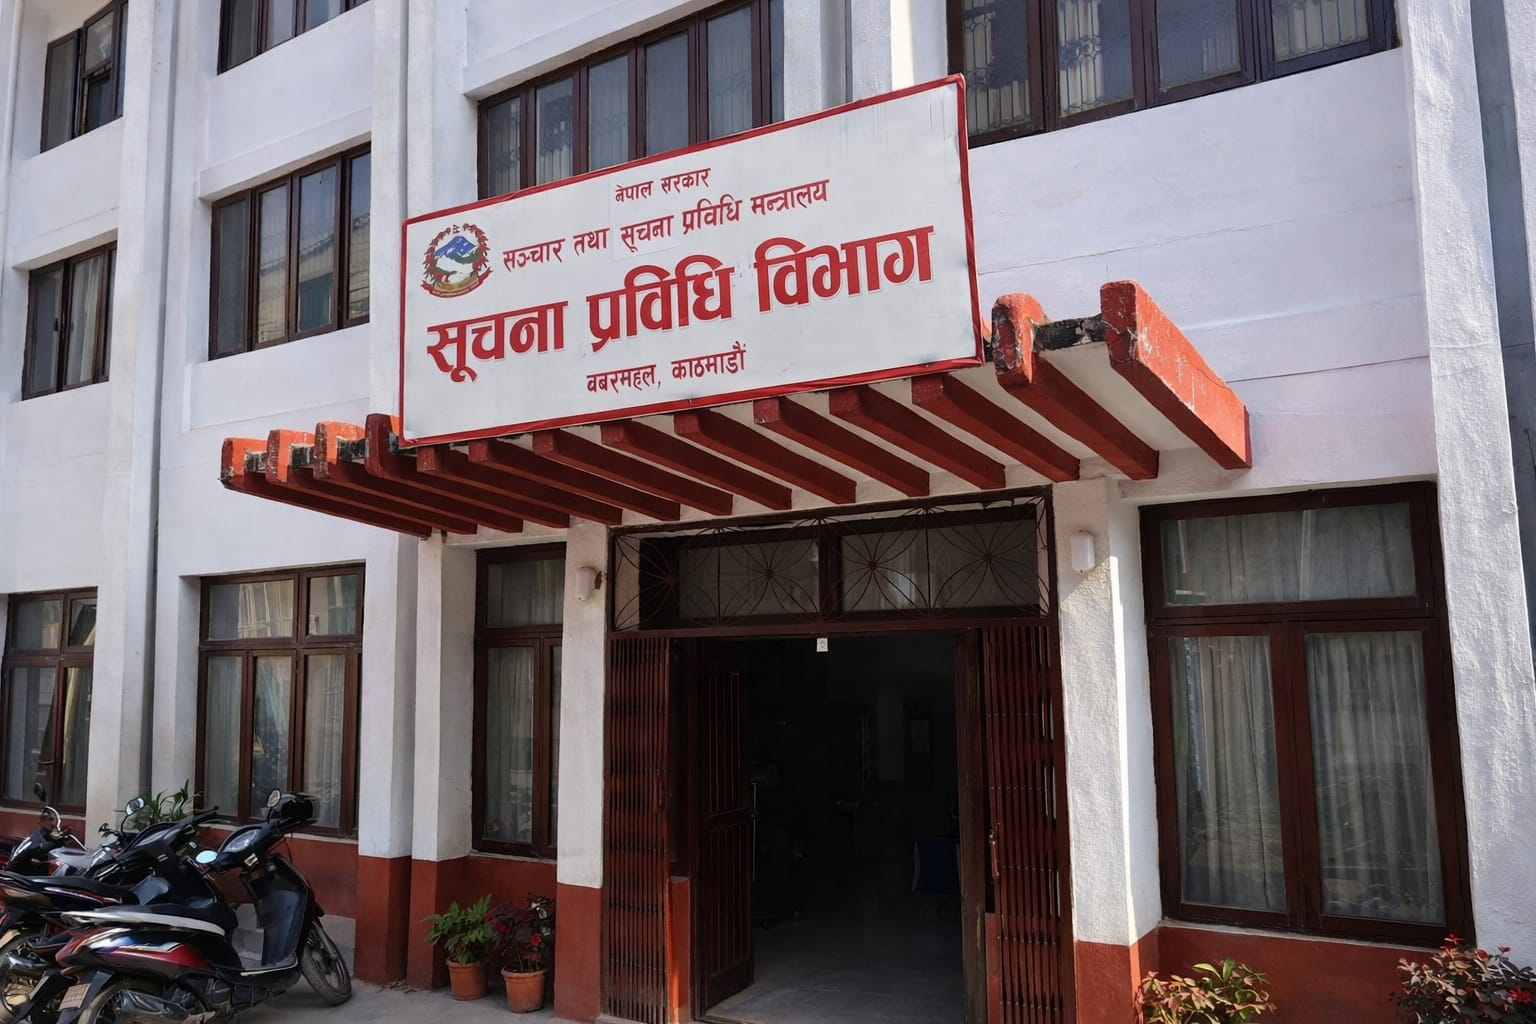
\includegraphics[width=0.85\textwidth]{MoICT.jpeg}
\caption{Information Technology Department , Ministry of Communication and Information Technology, Kathmandu - Field visit location, October 2025}
\end{figure}

\subsubsection{Figure 3: Research Team at Field Visit Site}

\begin{figure}[H]
\centering
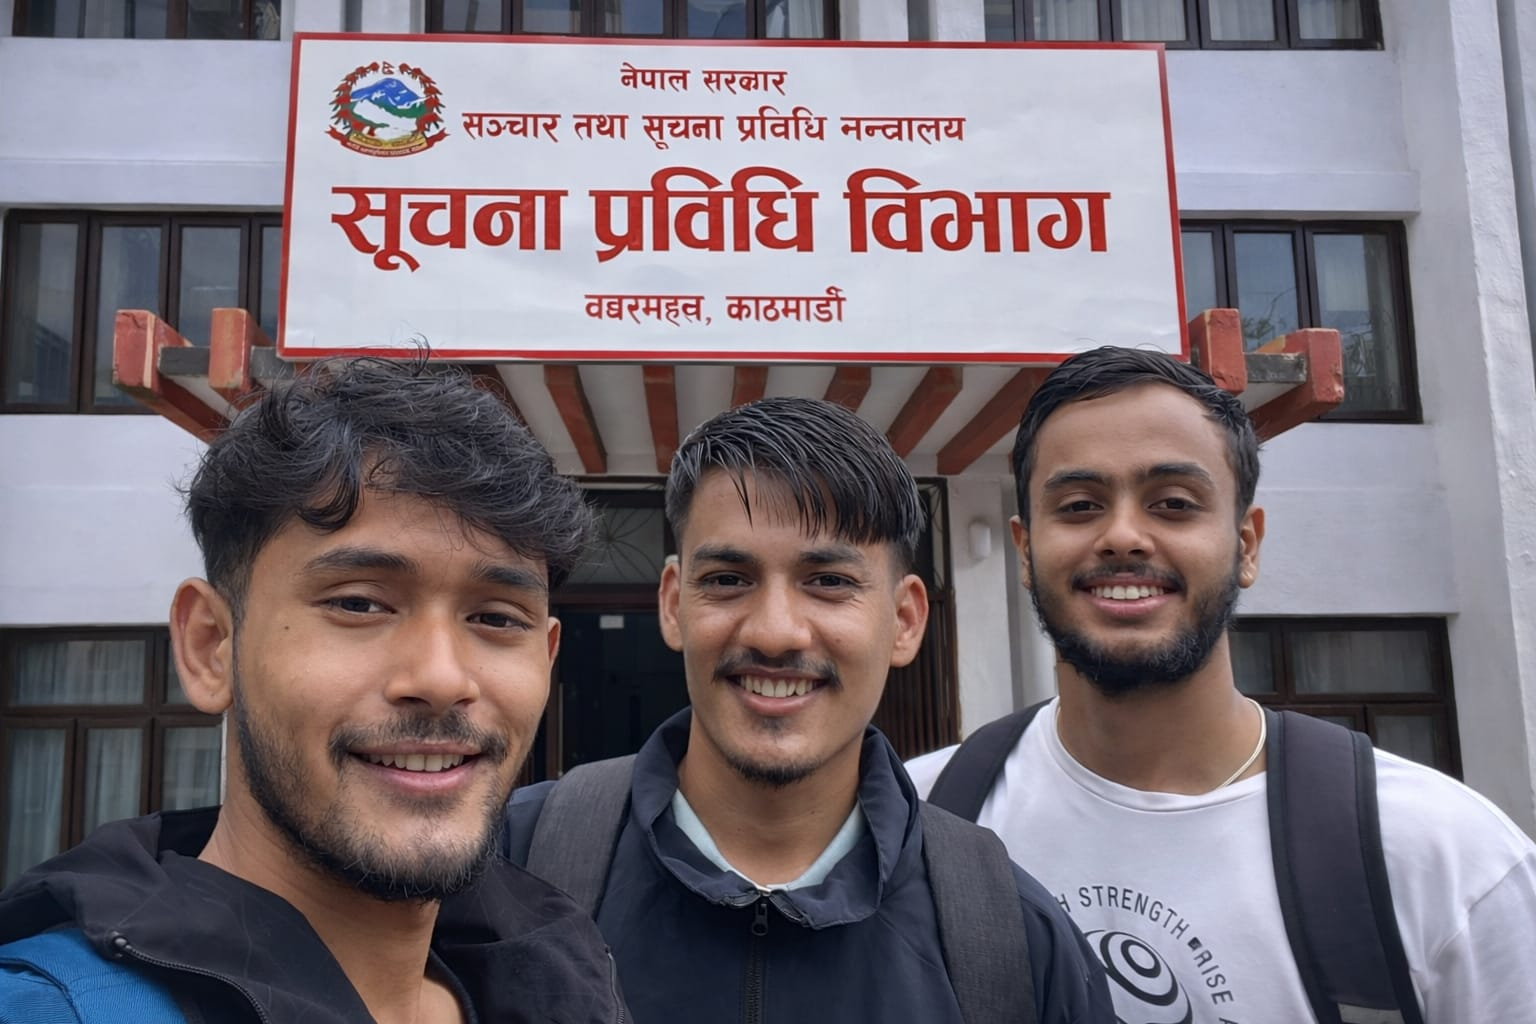
\includegraphics[width=0.85\textwidth]{selfie.jpeg}
\caption{Case study research team (Samir Paudel, Sachin Shrestha, and Umesh Bogati) at the Ministry of Communication and Information Technology during field visit for Digital Inclusion case study, October 2025}
\end{figure}

\subsection{Annexure E: Glossary of Terms}

\begin{description}
    \item[API (Application Programming Interface)] A set of protocols and tools for building software applications and enabling communication between different systems
    
    \item[BPR (Business Process Reengineering)] Fundamental rethinking and redesign of organizational processes to achieve improvements in performance
    
    \item[Digital Divide] The gap between those who have access to digital technologies and those who do not
    
    \item[Digital Literacy] The ability to use digital technologies effectively and responsibly
    
    \item[DNF (Digital Nepal Framework)] Nepal's strategic roadmap for digital transformation
    
    \item[DPI (Digital Public Infrastructure)] Foundational digital systems enabling government service delivery
    
    \item[E-governance] Use of ICT in government operations and service delivery
    
    \item[MoCIT] Ministry of Communication and Information Technology
    
    \item[Nagarik App] Nepal's integrated government services mobile application
    
    \item[NITC] National Information Technology Center
\end{description}

\end{document}
